\documentclass[runningheads]{llncs}
\usepackage[T1]{fontenc}
\usepackage{lmodern}
\usepackage{graphicx}
\usepackage{amsmath,amssymb}
\usepackage{booktabs}
\usepackage{microtype}
\usepackage{xcolor}
\usepackage[hidelinks]{hyperref}
\newcommand{\R}{\mathbb{R}}
\newcommand{\B}{\mathcal{B}}
\newcommand{\deltab}{\delta}
\renewcommand{\paragraph}[1]{\smallskip\noindent\textbf{#1}\ }

\begin{document}
\title{DIALS: Bundle Completion from Shared Relations Instead of Item Embeddings}
\titlerunning{DIALS: Bundle Completion from Shared Relations}
\author{Anonymous Submission}
\authorrunning{Anonymous}
\institute{Anonymous Institution}
\maketitle

% =====================================================================================================================
\begin{abstract}
Bundle completion asks a system to fill in the missing items of a partial bundle, such as an outfit or a playlist.
Current neural models learn an embedding for every item from the few bundles that contain it, so their size grows
with the catalogue and rarely bundled items are poorly described. We start from the observation that what makes items
go together is mostly shared across items: which categories or artists appear together, how similar two items are,
and how often they have been bundled. We propose DIALS, a model whose 41,624 parameters describe such relations and
never a single item. DIALS scores a candidate by a query-dependent weighted sum of content similarity, label
relations (a learned same-label term plus a low-rank term on fixed spectral factors) and discounted co-occurrence
counts. It is trained without leakage: each training bundle is scored with its own contribution removed from every
statistic. On seven datasets from fashion, music and e-commerce, we rerun two recent neural models on identical splits
and features and tune thirteen simple baselines. DIALS ranks the missing items better than every rerun neural model
and than the best simple baseline on all seven datasets (NDCG@20, Holm-corrected paired tests). A study of
training-set size shows where the learned model pays off: on playlists from 50 training bundles, on small e-commerce
bundles only from about 1,000, below which a training-free label and neighbourhood scorer is the better choice.
\keywords{bundle completion \and bundle construction \and recommender systems \and label relations}
\end{abstract}

% =====================================================================================================================
\section{Introduction}

A bundle is a set of items that are used together: an outfit of a top, trousers and shoes; a playlist built around a
few artists; a set of computer parts. Platforms rarely build bundles from nothing. A merchandiser picks one or two
products, or a listener adds a few songs, and the system is asked to suggest the rest. This is \emph{bundle
completion}: given some items of a bundle (the \emph{seeds}), rank the whole catalogue so that the missing items come
first (Fig.~\ref{fig:intro}a) \cite{clhe,ramen}. The task differs from user-based recommendation, because the query
is a set of items, not a user, and the answer must fit the seeds as a group.

Recent models treat bundle completion as representation learning. CLHE \cite{clhe} describes every item by an ID
embedding, multimodal features and a graph embedding, fuses them with self-attention, pools the seeds with a second
attention layer, and trains with reconstruction and contrastive losses. RaMen \cite{ramen} adds attention over an
item--item graph and a hypergraph of latent intents. Both score a candidate by an inner product between a bundle
vector and the candidate's item vector, and both learn part of that item vector from the bundles the item appears in.

This design ties what the model knows to individual items (Fig.~\ref{fig:intro}b). On our datasets CLHE has 0.75\,M
to 29\,M trained parameters and RaMen 1.3\,M to 67\,M, mostly rows of item tables. Each row is fitted only from the
bundles that contain its item, and bundle data are long-tailed: most items appear in a handful of bundles, and new
items in none. Large models are also hard to fit from such data, and their gains over well-tuned simple methods
should be checked, not assumed \cite{dacrema}.

Much of what makes items go together is not specific to an item. An outfit takes one item from each of several
categories and seldom two from the same one. A playlist does the opposite and returns to the same artists. Which label
goes with which is a relation among a few hundred labels, so every training bundle helps to learn it. Content
similarity and co-occurrence counts are also functions of item pairs that can be scored the same way for all items.
How much each kind of evidence should count depends on the query: a seed that occurs in many training bundles has
reliable co-occurrence counts, and a seed that occurs in none has only its content and its labels.

We build on this observation with \textbf{DIALS} (DIAgonal-plus-Low-rank label relations with Spectral cross-fitting).
DIALS scores a candidate by a gated sum of three kinds of evidence: content, label relations and co-occurrence
(Fig.~\ref{fig:intro}c). Its 41,624 parameters describe these relations, and none belongs to an item, so an item that
never appeared in a training bundle is scored by the same function as any other. Our contributions are:
\begin{itemize}
\item \textbf{A model with no per-item parameters.} Label relations are split into a learned same-label term, whose
sign is learned, and a low-rank term on fixed spectral factors of the label co-occurrence matrix, of which only a
$16\times16$ matrix is trained. Training removes each bundle's own contribution from every count and uses
cross-fitted factors, so the model never sees statistics that contain the answer.
\item \textbf{A matched comparison.} We rerun CLHE and RaMen with their own code on identical splits and identical
item features, with graphs built from training bundles only, and compare against thirteen tuned simple baselines,
four of which use the same labels as DIALS. DIALS is ahead of every rerun neural model and of the best simple
baseline on all seven datasets.
\item \textbf{Guidance on when a learned model pays off.} By training on 50 to all of the training bundles, we show
that DIALS leads from 50 playlists, but needs about 1,000 small e-commerce bundles; below that, a training-free
label and neighbourhood scorer is better, and the cause is overfitting rather than too few training steps.
\end{itemize}

\begin{figure}[t]
\centering
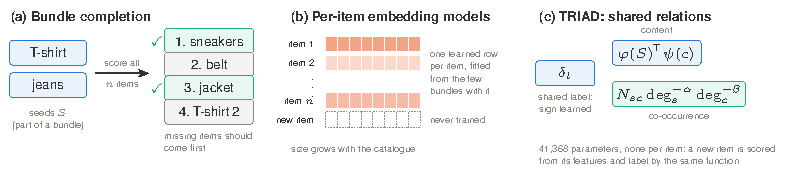
\includegraphics[width=\textwidth]{figs/fig1.pdf}
\caption{(a) Bundle completion ranks every catalogue item for a partial bundle. (b) Per-item models such as CLHE and
RaMen store part of their knowledge in one learned row per item. (c) DIALS learns relations that are shared by all
items: between labels, between item features, and over co-occurrence counts.}
\label{fig:intro}
\end{figure}

% =====================================================================================================================
\section{Related Work}

\paragraph{Bundle construction and completion.} Bundle recommendation ranks existing bundles for a user
\cite{bgcn,crosscbr}, and personalized bundle generation creates a bundle for a user \cite{bgn,pog}. Bundle
construction, the setting of this paper, starts from a partial bundle and has no user. CLHE \cite{clhe} and RaMen
\cite{ramen} learn item representations from several views and score candidates against a pooled seed vector.
Bundle-MLLM \cite{bundlemllm} fine-tunes a multimodal language model to pick the next item from a short candidate list,
and DDBC \cite{ddbc} generates bundles with discrete diffusion over item codes. Most of these models learn a
representation per item. DIALS learns none, and we compare against CLHE and RaMen directly.

\paragraph{Compatibility and complementarity.} Fashion compatibility models learn which items fit together, for
example from images \cite{han2017}, with separate spaces per category pair \cite{vasileva2018}, or as complements in
product graphs \cite{mcauley}. These works show that the relation between two items depends on their categories.
DIALS uses the same idea at the level of labels: it learns how strongly a seed's label supports a candidate's label,
including whether a shared label helps or hurts, which differs by domain (Section~\ref{sec:learned}).

\paragraph{Simple item-to-item methods.} Neighbourhood methods such as ItemKNN \cite{sarwar2001} and RP3$\beta$
\cite{rp3beta}, the linear model EASE \cite{steck2019} and graph filters such as GF-CF \cite{gfcf} and SGFCF
\cite{sgfcf} remain strong in recommendation, and several neural models have been found to trail them once they are
tuned \cite{dacrema,rendle2020}. RP3$\beta$ and the graph filters divide co-occurrence by item degree raised to a
tuned power; DIALS learns these powers. We tune these methods on validation and add label-aware variants, so that a
gain of DIALS cannot come from labels alone.

\paragraph{Leakage in training statistics.} When a model is trained on statistics computed from the same examples
it is trained on, each example sees a version of its own answer \cite{kapoor2023}. Cross-fitting, which computes a
nuisance quantity on other folds, is a standard remedy in statistics \cite{chernozhukov2018}. DIALS removes each
training bundle from its own counts exactly, and cross-fits the label factors, which cannot be corrected exactly.

% =====================================================================================================================
\section{Method}

\subsection{Task and notation}

The catalogue has $n$ items. Item $c$ has a feature vector $x_c\in\R^{d}$ ($X\in\R^{n\times d}$, rows normalized to
unit length) and, at each label level $l$, a label $g_l(c)$; the levels are the category for fashion and e-commerce,
and artist and album for music. From the training bundles $\B$ we count $N_{sc}$, the number of bundles that contain
both $s$ and $c$ ($s\neq c$), the item frequency $f_c$ (bundles that contain $c$) and the degree
$\deg_c=\sum_s N_{sc}$. A query is a seed set $S$, part of an unseen bundle; the task is to rank all items not in
$S$ so that the rest of the bundle comes first.

\subsection{Overview}

DIALS gives every item $c$ the score
\begin{equation}
s(c\mid S)=w_C(S)\,C(S,c)+\textstyle\sum_l w_l(S)\,L_l(S,c)+w_G(S)\,G(S,c),
\label{eq:score}
\end{equation}
the sum of a content term $C$, one label term $L_l$ per level and a graph term $G$, weighted by a gate $w(S)$ that
depends on the query (Fig.~\ref{fig:arch}). Each term answers one question about the candidate: does it look like it
belongs with the seeds, does its label go with the seeds' labels, and has it been bundled with the seeds before? The
three answers are useful at different times, which is why their weights depend on the query.

\begin{figure}[t]
\centering
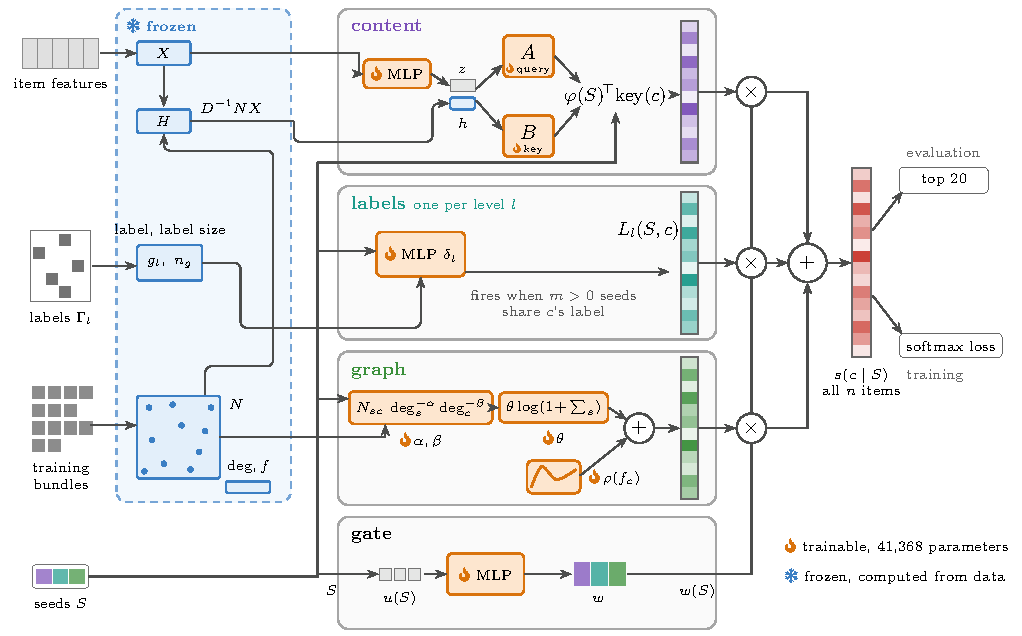
\includegraphics[width=\textwidth]{figs/fig2_arch.pdf}
\caption{DIALS. Frozen structures (blue) are computed once from the item features, labels and training bundles.
Each term (content, labels, graph) gives a score vector over all $n$ items; the gate weights them per query, and their
sum ranks the catalogue. All 41,624 trained parameters (orange) are shared by all items.}
\label{fig:arch}
\end{figure}

\subsection{Content}

The content term compares the seeds with the candidate through learned low-rank maps. Item features are first refined
by a small residual network, $Z=\mathrm{normalize}(X+\mathrm{MLP}(X))$. Each item also gets a \emph{partner history}
$h_c$, the count-weighted mean feature of the items it has been bundled with: $H=\mathrm{diag}(\deg)^{-1}NX$. The
history describes an item by what it has been bundled with, not only by what it is. Then
\begin{equation}
C(S,c)=\varphi(S)^{\top}\psi(c),\ \ \varphi(S)=\tfrac{1}{|S|}\textstyle\sum_{s\in S}(A_z z_s+A_h h_s),\ \
\psi(c)=B_z z_c+B_h h_c
\end{equation}
with $A_z,A_h,B_z,B_h\in\R^{64\times d}$. Separate seed-side ($A$) and candidate-side ($B$) maps let the score be
asymmetric: a jacket can call for boots without boots calling for a jacket. The maps start at a scaled identity on
the first 64 feature coordinates, so training starts from plain feature similarity.

\subsection{Labels: diagonal plus low rank}

Let $t(S)\in\R^{K}$ count how many seeds carry each of the $K$ labels of a level. A natural score is a $K\times K$
table $R$, where $R_{gg'}$ says how well a seed with label $g$ supports a candidate with label $g'$:
$L(S,c)=\tfrac{1}{|S|}t(S)^{\top}R\,e_{g(c)}$. With $K$ up to 116,217 on Spotify (albums), $R$ cannot be learned
freely. DIALS splits it into a diagonal and a low-rank part, $R=\Delta+P M Q^{\top}$, which do different jobs.

\paragraph{Same label (the diagonal).} The diagonal entry $R_{gg}$ scores a candidate whose label is shared by
$m=t_{g(c)}(S)$ seeds. A fixed diagonal would give $m\,\Delta_{gg}$. DIALS lets the value depend on how many seeds
share the label, on the query size and on how large the label is ($n_g$ items):
$\deltab_l(\log(1+m),\log|S|,\log(1+n_{g(c)}))\cdot[m>0]$, where $\deltab_l$ is an MLP with 16 hidden units shared by
all labels. Its output can be negative, so the model can learn that sharing a label is evidence against a candidate.
Sharing a small label is a strong hint, while sharing a large one (``shoes'') says little, which is why $n_g$ is an
input.

\paragraph{Related labels (the low rank).} The off-diagonal part says which different labels go together, such as
skirts with sandals. We take it from the data: with $\Gamma\in\{0,1\}^{n\times K}$ the item-to-label matrix,
$\bar N=\Gamma^{\top}N\Gamma$ counts how often two labels share a bundle. After normalizing by the label degrees,
$\hat N=D^{-1/2}\bar N D^{-1/2}$ with $D=\mathrm{diag}(\max(\bar N\mathbf{1},1))$, a rank-16 truncated SVD
$\hat N\approx U\Sigma V^{\top}$ gives fixed factors $P=U\Sigma^{1/2}$ and $Q=V\Sigma^{1/2}$ ($K\times16$). Only
$M\in\R^{16\times16}$ is learned, starting at zero. The SVD provides a compact coordinate system for labels from the
counts; $M$ learns how much each direction should count and with which sign. Every item in a label gets the same
low-rank score, so a new item is scored through its label.

\subsection{Graph}

The graph term uses direct co-occurrence with the seeds, discounted for items that are bundled with everything:
\begin{equation}
G(S,c)=\theta\log\Big(1+\textstyle\sum_{s\in S}N_{sc}\deg_s^{-\alpha}\deg_c^{-\beta}\Big)+\rho\big(\log(1+f_c)\big),
\end{equation}
with learned $\theta,\alpha,\beta$ and a small MLP $\rho$ that learns a popularity prior. Only the stored non-zero
counts of the seeds' rows are read, so the cost per query is the number of the seeds' partners, not $n$.

\subsection{Gate}

The gate reads three statistics of the query: its size $\log|S|$, the mean seed frequency
$\tfrac{1}{|S|}\sum_{s\in S}\log(1+f_s)$ and the share of seeds with $f_s=0$. From these $u(S)$ it returns the weights $w(S)=\mathrm{softplus}(\mathrm{MLP}(u(S)))$, one per term. A query
whose seeds were never bundled has no co-occurrence evidence, and the gate can move weight to content and labels.

\subsection{Training without leakage}

\paragraph{Examples and loss.} Each step takes 32 training bundles and hides a random part of each: half of the items
with probability $1/2$, otherwise a uniform cut, so that queries of all sizes are seen. The visible items are the
seeds. Each hidden item $j$ competes with all catalogue items outside its bundle through the loss
$\mathrm{softplus}(\mathrm{LSE}_{c\notin b}\,s(c\mid S)-s(j\mid S))$, averaged over hidden items.

\paragraph{Leave-one-out statistics.} A training bundle $b$ is part of $N$, $f$, $\deg$ and $H$. If it stayed there,
the counts between its seeds and its hidden items would contain the answer, and the model would learn to trust
co-occurrence far more than it should at test time, where no such count exists. So each training bundle is scored
with its own contribution removed: $N_{sc}-1$ for pairs inside $b$, $\deg-(|b|-1)$ and $f-1$ for its members, and
the same correction in $H$. Only the counts of the seeds' rows are touched, so the correction is cheap.

\paragraph{Cross-fitted label factors.} The SVD factors cannot be corrected exactly for one bundle. The training
bundles are therefore split into five folds (identical bundles share a fold), and a bundle in fold $k$ is scored
with factors computed without fold $k$. Evaluation uses factors from all training bundles.

\paragraph{One configuration.} Content rank 64, label rank 16, AdamW with learning rate $10^{-2}$ for the small
relation parameters and $10^{-3}$ for the content maps, weight decay $10^{-3}$, early stopping on validation NDCG@20
with patience 6 and at most 100 epochs. Nothing is tuned per dataset. The model has 41,624 parameters, 41,978 with two
label levels, independent of $n$.

% =====================================================================================================================
\section{Experiments}

We ask four questions. Does DIALS rank the missing items better than neural and simple baselines under one protocol
(Section~\ref{sec:main})? Which parts matter (Section~\ref{sec:ablation})? How much training data does it need
(Section~\ref{sec:budget})? And what does it learn (Section~\ref{sec:learned})?

\subsection{Setup}

\paragraph{Datasets.} We use the seven public datasets that come with real bundles (Table~\ref{tab:data}). POG and
POG\_DENSE are outfits from Alibaba iFashion \cite{pog}, and Spotify and Spotify\_sparse are playlists from the RecSys
Challenge 2018 \cite{spotify}, all with the train, validation and test files released with CLHE \cite{clhe}, used
unchanged. Each test bundle comes split into seeds and held-out items. Electronic, Food and Clothing are product
bundles released by Sun et al.\ \cite{bundlerec}; we remove duplicate bundles, split them 70/10/20 with a fixed seed
and hide half of each validation and test bundle. Item features are the released ones, the same for every method:
BLIP image and text embeddings \cite{blip} for POG and CLAP audio and text embeddings \cite{clap} for Spotify. The
e-commerce data have no released features, so we use TF-IDF of the item titles. All features are projected to 128
dimensions by a truncated SVD.

\begin{table}[t]
\centering
\caption{Datasets. Size: mean items per training bundle. Labels: values per level (category; artist, album).
Test: test queries, with clean ones in brackets when some test bundles also occur in training or validation.}
\label{tab:data}
\setlength{\tabcolsep}{4pt}
\small
\begin{tabular}{llrrrrl}
\toprule
Domain & Dataset & Items & Train & Size & Test & Labels\\
\midrule
E-commerce & Electronic & 3,499 & 1,211 & 3.5 & 346 & 479\\
 & Food & 3,767 & 1,232 & 3.5 & 353 & 836\\
 & Clothing & 4,487 & 1,294 & 3.3 & 371 & 2,033\\
Fashion & POG\_DENSE & 31,217 & 20,780 & 3.6 & 5,938 (5,547) & 67\\
 & POG & 48,676 & 14,000 & 3.6 & 4,000 (3,995) & 72\\
Music & Spotify\_sparse & 213,325 & 8,740 & 44.2 & 2,498 (2,497) & 43,039; 98,674\\
 & Spotify & 254,155 & 14,000 & 63.6 & 4,000 (3,995) & 49,164; 116,217\\
\bottomrule
\end{tabular}
\end{table}

\paragraph{Protocol.} Every method ranks the full catalogue with the seeds removed, and we report Recall@20 and
NDCG@20. Some released test bundles of POG and Spotify also occur, complete, in the training or validation files; a
method that memorizes bundles gets them for free, so we report \emph{clean} test queries, which exclude them
(Table~\ref{tab:data}). Learned models are run with seeds 0, 1 and 2, and per-query metrics are averaged over seeds.
Differences come with a 95\% paired bootstrap interval and a paired sign-flip test, both resampling clusters of
identical bundles, with Holm's correction within each table.

\paragraph{Baselines.} \emph{Simple:} popularity, co-occurrence, ItemKNN \cite{sarwar2001}, RP3$\beta$
\cite{rp3beta}, EASE \cite{steck2019}, GF-CF \cite{gfcf}, SGFCF \cite{sgfcf}, iALS \cite{hu2008}, a blend of ItemKNN
with content cosine, and four label-aware methods that use DIALS's labels: same-label counts, label transition
probabilities, and the better of the two blended with ItemKNN, with and without content (EASE is too large for
Spotify). Every method is tuned on validation NDCG@20, and the best one per dataset is chosen on validation as well. \emph{Neural:} CLHE \cite{clhe} and RaMen \cite{ramen},
run with the authors' code and settings chosen on validation. Both use the same item features as DIALS. Their user or
item graphs are built from training bundles only, the information DIALS has. RaMen's item--item graph builder is not
released, so we rebuilt it from the paper. On full Spotify, CLHE ran at batch size 128 instead of 256 to fit in GPU
memory, and only one of three seeds finished within the 12-hour limit, so it is not tested there. We did not rerun
RaMen on POG and Spotify and quote its published numbers, which use the same split files.

\subsection{Main results}
\label{sec:main}

\begin{table}[t]
\centering
\caption{Recall@20 / NDCG@20 on clean test queries (mean of three seeds). Best simple: the baseline chosen on
validation (cont.+kNN: content+ItemKNN blend; lab.+kNN+cont.: label+ItemKNN+content). $\Delta$: DIALS minus best simple in NDCG@20, with a 95\% interval. All 14 DIALS--best-simple tests
(7 datasets $\times$ 2 metrics) and all 12 DIALS--CLHE and 6 DIALS--RaMen tests reject at $p<0.05$ after Holm.
$^\dagger$Published number on the same split files, all test queries, not rerun. $^\ddagger$One seed, not tested.}
\label{tab:main}
\setlength{\tabcolsep}{3pt}
\resizebox{\textwidth}{!}{%
\small
\begin{tabular}{lllllll}
\toprule
Dataset & Best simple & & CLHE & RaMen & DIALS & $\Delta$ NDCG [CI]\\
\midrule
Electronic & cont.+kNN & .432 / .299 & .362 / .260 & .344 / .254 & \textbf{.469 / .335} & +.036 [.016, .057]\\
Food & lab.+kNN+cont. & .546 / .412 & .370 / .272 & .352 / .274 & \textbf{.586 / .439} & +.027 [.008, .048]\\
Clothing & lab.+kNN+cont. & .446 / .333 & .241 / .186 & .238 / .191 & \textbf{.534 / .388} & +.055 [.033, .078]\\
POG\_DENSE & RP3$\beta$ & .345 / .241 & .349 / .248 & -- & \textbf{.376 / .280} & +.040 [.036, .043]\\
POG & lab.+kNN+cont. & .036 / .023 & .026 / .017 & .038 / .023$^\dagger$ & \textbf{.054 / .031} & +.008 [.006, .010]\\
Spotify\_sparse & lab.+kNN+cont. & .147 / .205 & .097 / .115 & -- & \textbf{.184 / .256} & +.051 [.046, .056]\\
Spotify & lab.+kNN+cont. & .147 / .247 & (.179)$^\ddagger$ & .109 / .188$^\dagger$ & \textbf{.167 / .282} & +.036 [.031, .040]\\
\midrule
\multicolumn{2}{l}{Trained parameters} & -- & 0.75\,M--29\,M & 1.3\,M--67\,M & 41.6\,k & \\
\bottomrule
\end{tabular}}
\end{table}

Table~\ref{tab:main} gives the results. Three things stand out.

\paragraph{DIALS is ahead on every dataset.} Against the best simple baseline the gap in NDCG@20 ranges from +.008
on POG to +.055 on Clothing, and every interval excludes zero. The smallest margins are on Food (+.027) and POG
(+.008, on a dataset where all methods score low).

\paragraph{Tuned simple baselines are strong.} The best simple baseline is ahead of CLHE on five of the six datasets
where CLHE was rerun; on POG\_DENSE, CLHE is slightly ahead. On e-commerce, CLHE and RaMen trail the best simple
baseline by .04--.15 NDCG@20. This agrees
with earlier findings in recommendation \cite{dacrema}, and it means that a gain over CLHE or RaMen alone says little.

\paragraph{Labels help simple methods too, but do not explain DIALS's lead.} A label-aware method is the best simple
baseline on five datasets, so labels carry real signal. DIALS uses the same labels and still leads each of them.

\paragraph{About published e-commerce numbers.} RaMen reports Recall@20 of .837 on Electronic and .846 on Food
\cite{ramen} on a split that is not released. Its released user--item file contains the items of every bundle,
test bundles included, so a graph built from it links each test target to its seeds. Rerun on our split with that
file, RaMen reaches .499 / .489 / .483 Recall@20 on Electronic / Food / Clothing, against .344 / .352 / .238 with a
graph from training bundles only. We report the latter, which uses the same information as every other method.

\paragraph{Cost.} DIALS has no per-item parameters and needs 0.1\,ms per query on e-commerce, 0.4--0.5\,ms on POG and
2.4--3.2\,ms on Spotify on four CPU threads, after a one-time computation of the counts and label factors.

\subsection{Ablations}
\label{sec:ablation}

We retrain DIALS with one part removed at a time, with the same configuration and seeds, on the six datasets other
than full Spotify, where one training run takes 1--1.5\,h of CPU time (Table~\ref{tab:ablation}).

\begin{table}[t]
\centering
\caption{Ablations: NDCG@20 of the full model minus the ablated model, clean test queries, three seeds. Positive:
the part helps. Bold: Holm-corrected $p<0.05$ (12 tests per row). [TO BE FILLED WHEN THE RUNS FINISH]}
\label{tab:ablation}
\setlength{\tabcolsep}{3pt}
\scriptsize
\begin{tabular}{lcccccc}
\toprule
Removed part & Electronic & Food & Clothing & POG\_DENSE & POG & Spotify\_sparse\\
\midrule
same-label diagonal $\deltab_l$ & & & & & & \\
related-label low rank ($M=0$) & & & & & & \\
cross-fitting of $P,Q$ & & & & & & \\
leave-one-out statistics & & & & & & \\
gate (all weights 1) & & & & & & \\
content term & & & & & & \\
label terms & & & & & & \\
graph term & & & & & & \\
training (initial parameters) & & & & & & \\
\bottomrule
\end{tabular}
\end{table}

\subsection{How much training data does DIALS need?}
\label{sec:budget}

A retailer that starts with bundle completion has few example bundles. We train DIALS and retune every simple
baseline on nested random subsets of the training bundles (3,000, 1,000, 600, 300, 100 and 50; POG and POG\_DENSE at
10\% and 1\%), with the same validation and test queries. For each subset we retune ten of the simple baselines (all but GF-CF,
SGFCF and iALS) and compare DIALS with the one chosen on validation (Fig.~\ref{fig:budget}).

\begin{figure}[t]
\centering
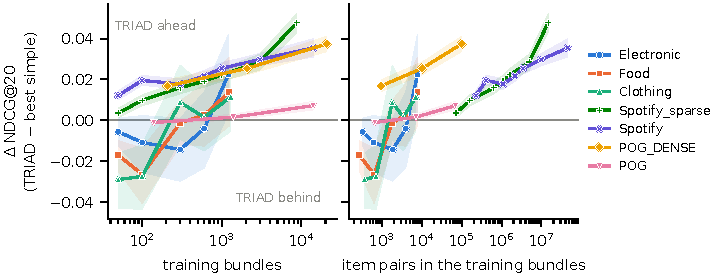
\includegraphics[width=.92\textwidth]{figs/fig3_budget.pdf}
\caption{DIALS minus the best simple baseline (NDCG@20, clean test, 95\% interval) as training bundles are removed,
against the number of bundles (left) and the number of item pairs they contain (right).}
\label{fig:budget}
\end{figure}

\paragraph{Playlists: DIALS leads at every size.} On Spotify and Spotify\_sparse, DIALS stays ahead down to 50
playlists (+.012 and +.004 NDCG@20), and all 28 tests reject after Holm. The lead shrinks steadily as bundles are
removed.

\paragraph{Small e-commerce bundles: DIALS needs about 1,000.} On Electronic, Food and Clothing, DIALS is ahead with
all of their 1,200--1,300 bundles, level with 600, and behind with 300 or fewer, by .03--.09 NDCG@20. All nine
intervals at 300 and below lie under zero.

\paragraph{The cause is overfitting.} Two checks on the e-commerce subsets point the same way. Repeating the bundles
so that each epoch has as many gradient steps as on the full data does not help: validation NDCG peaks after one to
six epochs and then falls while the training loss keeps dropping (Food, 50 bundles: loss 6.47 to 0.43, validation
NDCG .167 to .114). The untrained model, at its initial parameters, scores below the trained one in eight of nine
cases, so training helps, but it does not reach the tuned label+ItemKNN+content scorer before it overfits.

\paragraph{What predicts the outcome.} Bundle count alone does not: 50 playlists are enough, 300 product bundles are
not. A playlist holds about 1,700--3,300 item pairs, a product bundle about 6, so 50 playlists contain more pairs than
all e-commerce training sets (Fig.~\ref{fig:budget}, right). Pairs alone do not decide it either: POG\_DENSE at 1\%
(952 pairs) still favours DIALS, because 34\% of its test targets occur in those bundles. In our data, DIALS fell
behind only when both were small, under about 2,000 pairs and at most 28\% of test targets seen. This is an
observation on seven datasets, not a tested rule. For practice it suggests: with long bundles, train DIALS from the
start; with short bundles and fewer than about 1,000 of them, use a tuned label+ItemKNN+content scorer.

\subsection{What DIALS learns}
\label{sec:learned}

\begin{figure}[t]
\centering
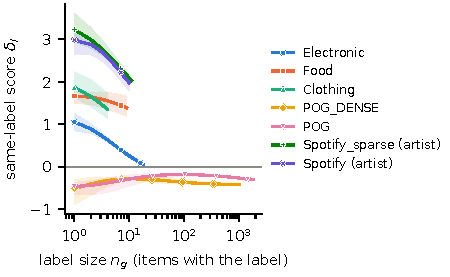
\includegraphics[width=.62\textwidth]{figs/fig4_delta.pdf}
\caption{The learned same-label score $\deltab_l$ for one shared seed ($m=1$) at the median query size, against the
size of the label (mean of three seeds, band: min to max). It is negative for fashion and positive for music and
e-commerce.}
\label{fig:delta}
\end{figure}

The same-label term $\deltab_l$ starts as a small random MLP, and its sign is not fixed. After training it differs
by domain (Fig.~\ref{fig:delta}). On POG and POG\_DENSE it is negative for every label size: an outfit rarely takes
two items of the same category, so sharing a seed's category counts against a candidate. On Spotify it is strongly
positive for small artists: playlists return to the same artist, and an artist with few songs is a sharp signal. On
e-commerce, where the labels are fine-grained, a shared label helps when the label is small and the bonus fades for
large labels. One configuration recovers these opposite patterns from the data alone.

% =====================================================================================================================
\section{Conclusion}

We showed that bundle completion does not need a learned representation per item. DIALS learns 41,624 shared
parameters that weight content similarity, label relations and co-occurrence for each query, and is trained with
statistics that never contain the training bundle itself. Under one protocol, with neural models rerun on identical
splits and features, it ranks missing items better than CLHE, RaMen and thirteen tuned simple baselines on seven
datasets, and its learned label relations are readable.

\paragraph{Limitations.} The margins over the best simple baseline are small on POG and Food. On short e-commerce
bundles, DIALS needs about 1,000 training bundles, and a training-free scorer is better below that. Although DIALS can
score new items, features find unseen POG targets only at chance level, so new items remain hard. Scoring is linear
in the catalogue size, so catalogues of millions of items would need a candidate stage. Finally, two of our baseline
numbers are published, not rerun.

\paragraph{Future work.} A natural next step is to start training from the tuned simple scorer and penalize moving
away from it, which may remove the small-data gap. Code will be released.

\begin{thebibliography}{99}\scriptsize
\bibitem{bgn} Bai, J., Zhou, C., Song, J., Qu, X., An, W., Li, Z., Gao, J.: Personalized bundle list recommendation. In: WWW (2019)
\bibitem{blip} Li, J., Li, D., Xiong, C., Hoi, S.: BLIP: Bootstrapping language-image pre-training for unified vision-language understanding and generation. In: ICML (2022)
\bibitem{bgcn} Chang, J., Gao, C., He, X., Jin, D., Li, Y.: Bundle recommendation with graph convolutional networks. In: SIGIR (2020)
\bibitem{pog} Chen, W., et al.: POG: Personalized outfit generation for fashion recommendation at Alibaba iFashion. In: KDD (2019)
\bibitem{spotify} Chen, C.W., Lamere, P., Schedl, M., Zamani, H.: RecSys Challenge 2018: Automatic music playlist continuation. In: RecSys (2018)
\bibitem{chernozhukov2018} Chernozhukov, V., Chetverikov, D., Demirer, M., Duflo, E., Hansen, C., Newey, W., Robins, J.: Double/debiased machine learning for treatment and structural parameters. The Econometrics Journal 21(1), C1--C68 (2018)
\bibitem{dacrema} Ferrari Dacrema, M., Cremonesi, P., Jannach, D.: Are we really making much progress? A worrying analysis of recent neural recommendation approaches. In: RecSys (2019)
\bibitem{han2017} Han, X., Wu, Z., Jiang, Y.G., Davis, L.S.: Learning fashion compatibility with bidirectional LSTMs. In: ACM MM (2017)
\bibitem{hu2008} Hu, Y., Koren, Y., Volinsky, C.: Collaborative filtering for implicit feedback datasets. In: ICDM (2008)
\bibitem{kapoor2023} Kapoor, S., Narayanan, A.: Leakage and the reproducibility crisis in machine-learning-based science. Patterns 4(9) (2023)
\bibitem{bundlemllm} Liu, X., Wu, J., Tao, Z., Ma, Y., Wei, Y., Chua, T.S.: Fine-tuning multimodal large language models for product bundling. In: KDD (2025)
\bibitem{crosscbr} Ma, Y., He, Y., Zhang, A., Wang, X., Chua, T.S.: CrossCBR: Cross-view contrastive learning for bundle recommendation. In: KDD (2022)
\bibitem{clhe} Ma, Y., Liu, X., Wei, Y., Tao, Z., Wang, X., Chua, T.S.: Leveraging multimodal features and item-level user feedback for bundle construction. In: WSDM (2024)
\bibitem{mcauley} McAuley, J., Pandey, R., Leskovec, J.: Inferring networks of substitutable and complementary products. In: KDD (2015)
\bibitem{ramen} Nguyen, H.S., Nguyen, Q.H., Pham, D.H., Le, D.T., Le, H.Q., Sitkrongwong, P., Takasu, A., Mansoury, M.: RaMen: Multi-strategy multi-modal learning for bundle construction. In: ECAI (2025)
\bibitem{rp3beta} Paudel, B., Christoffel, F., Newell, C., Bernstein, A.: Updatable, accurate, diverse, and scalable recommendations for interactive applications. ACM TiiS 7(1) (2017)
\bibitem{sgfcf} Peng, S., Liu, X., Sugiyama, K., Mine, T.: How powerful is graph filtering for recommendation. In: KDD (2024)
\bibitem{rendle2020} Rendle, S., Krichene, W., Zhang, L., Anderson, J.: Neural collaborative filtering vs. matrix factorization revisited. In: RecSys (2020)
\bibitem{sarwar2001} Sarwar, B., Karypis, G., Konstan, J., Riedl, J.: Item-based collaborative filtering recommendation algorithms. In: WWW (2001)
\bibitem{gfcf} Shen, Y., Wu, Y., Zhang, Y., Shan, C., Zhang, J., Letaief, K.B., Li, D.: How powerful is graph convolution for recommendation? In: CIKM (2021)
\bibitem{steck2019} Steck, H.: Embarrassingly shallow autoencoders for sparse data. In: WWW (2019)
\bibitem{bundlerec} Sun, Z., Feng, K., Yang, J., Fang, H., Qu, X., Ong, Y.S., Liu, W.: Revisiting bundle recommendation for intent-aware product bundling. ACM TORS 2(3) (2024)
\bibitem{ddbc} Tu, T., Li, A., Ma, Y., Xu, S., Liu, X., Ma, H., Pang, L., Chua, T.S.: Discrete diffusion for bundle construction. In: ICLR (2026)
\bibitem{vasileva2018} Vasileva, M.I., Plummer, B.A., Dusad, K., Rajpal, S., Kumar, R., Forsyth, D.: Learning type-aware embeddings for fashion compatibility. In: ECCV (2018)
\bibitem{clap} Wu, Y., Chen, K., Zhang, T., Hui, Y., Berg-Kirkpatrick, T., Dubnov, S.: Large-scale contrastive language-audio pretraining with feature fusion and keyword-to-caption augmentation. In: ICASSP (2023)
\end{thebibliography}
\end{document}
